\documentclass[tikz,border=5pt]{standalone}
\usepackage{amsmath}
\begin{document}
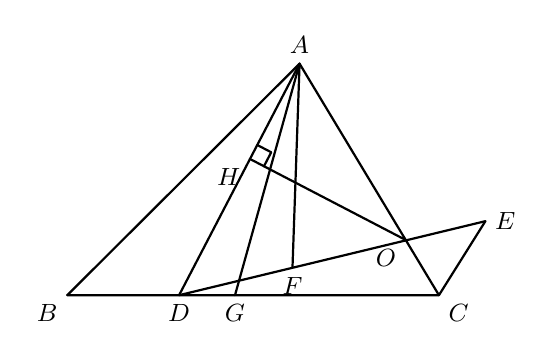
\begin{tikzpicture}[line cap=round, line join=round, font=\small]
  % Coordinates (cm)
  \coordinate (A) at (3.65,2.94);
  \coordinate (B) at (0.70,0);
  \coordinate (C) at (5.42,0);
  \coordinate (D) at (2.12,0);
  \coordinate (G) at (2.83,0);
  \coordinate (F) at (3.56,0.35);
  \coordinate (E) at (6.01,0.94);
  \coordinate (O) at (5.00,0.70);
  \coordinate (H) at (3.02,1.73);

  % Original figure elements
  \draw[thick] (B) -- (A) -- (C) -- cycle;
  \draw[thick] (B) -- (C);
  \draw[thick] (A) -- (D);
  \draw[thick] (A) -- (G);
  \draw[thick] (A) -- (F);
  \draw[thick] (D) -- (E);
  \draw[thick] (C) -- (E);

  % Perpendicular from O to AD
  \draw[thick] (O) -- (H);

  % Right angle mark at H
  \draw[thick] (3.1127,1.9076) -- (3.2899,1.8150) -- (3.1976,1.6376);

  % Point labels
  \node[above] at (A) {$A$};
  \node[below left] at (B) {$B$};
  \node[below right] at (C) {$C$};
  \node[below] at (D) {$D$};
  \node[below] at (G) {$G$};
  \node[below] at (F) {$F$};
  \node[right] at (E) {$E$};
  \node[below left] at (O) {$O$};
  \node[below left] at (H) {$H$};
\end{tikzpicture}
\end{document}
